\documentclass[border=0.25cm]{standalone}
\usepackage{xcolor}
\usepackage{tikz}
\usetikzlibrary{arrows, arrows.meta}
\tikzset{    
    barbarrow/.style={ 
        color=blue,
        % style that just defines the arrow tip
        >={Straight Barb[left,length=5pt,width=5pt]},
        thick,
        <->
    },
    blues/.style={
        color=blue
    },
    reds/.style={
        color=red
    }
}
\definecolor{light-gray}{gray}{0.975}
\definecolor{pcolor}{rgb}{0.21, 0.27, 0.31}
\begin{document}
\begin{tabular}{c c c c c}
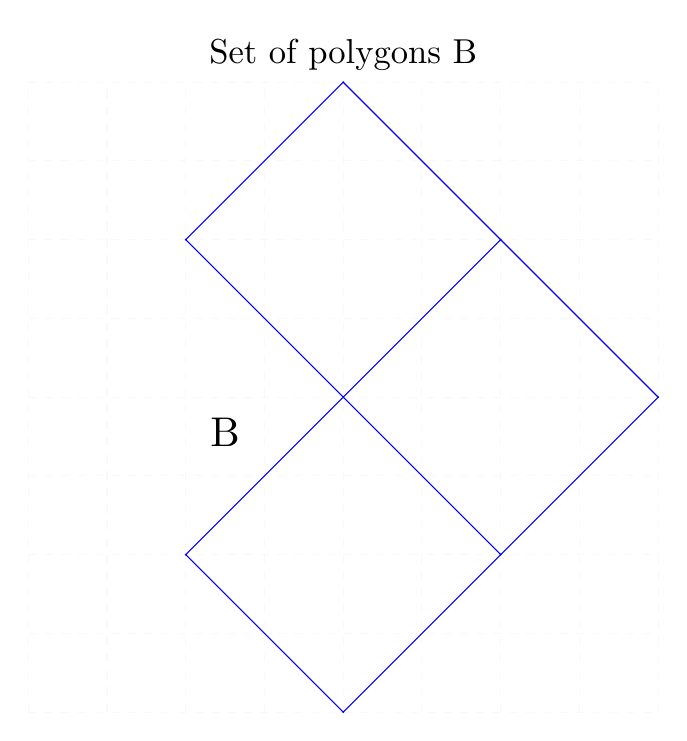
\begin{tikzpicture}
    \tikzstyle{node1}=[draw,scale=0.02,shape=circle,color=blue,fill=blue]
    \draw[color=light-gray, style=dashed] (0,0) grid (8,8);
    \node[above, scale=1.25] at (4,8) {Set of polygons B};
    \node[node1] (D) at (2,2) {};
    \node[node1] (F) at (2,6) {};
    \node[node1] (J) at (4,0) {};
    \node[node1] (L) at (4,4) {};
    \node[node1] (N) at (4,8) {};
    \node[node1] (Q) at (6,2) {};
    \node[node1] (S) at (6,6) {};
    \node[node1] (T) at (8,4) {};
    \node[scale=1.5] at (2.5,3.55) {B};    
    
    \draw[blues] 
        (D) -- (J) (D) -- (L) (F) -- (N) (F) -- (L) (J) -- (Q) 
        (L) -- (Q) (L) -- (S) (N) -- (S) (Q) -- (T) (S) -- (T);
\end{tikzpicture} 
&
\begin{tikzpicture}
    \draw[color=white, style=dashed] (0,0) grid (0,8);
    \node[scale=4] at (0, 4) {$\Longrightarrow$};
\end{tikzpicture} 
&
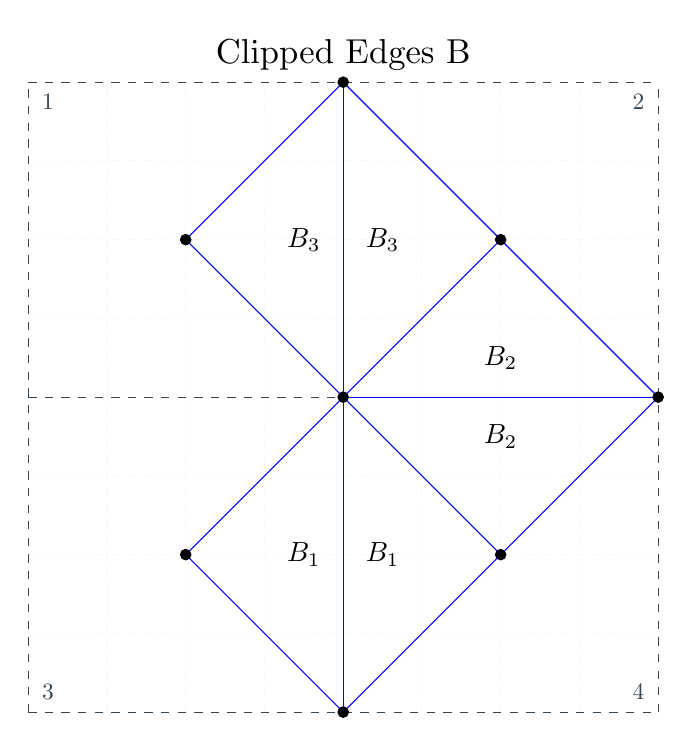
\begin{tikzpicture}
    \tikzstyle{node1}=[draw,scale=0.4,shape=circle,color=black,fill=black]
    \tikzstyle{node2}=[draw,scale=0.4,shape=circle,color=red,fill=red]    
    \draw[color=light-gray, style=dashed] (0,0) grid (8,8);
    \draw[color=pcolor, style=dashed, step=4] (0,0) grid (8,8);
    \node[scale=0.85, color = pcolor] at (0.25, 7.75) {$1$};
    \node[scale=0.85, color = pcolor] at (7.75, 7.75) {$2$};
    \node[scale=0.85, color = pcolor] at (0.25, 0.25) {$3$};
    \node[scale=0.85, color = pcolor] at (7.75, 0.25) {$4$};
    
    \node[above, scale=1.25] at (4,8) {Clipped Edges B};
    \node[node1] (D) at (2,2) {};
    \node[node1] (F) at (2,6) {};
    \node[node1] (J) at (4,0) {};
    \node[node1] (L) at (4,4) {};
    \node[node1] (N) at (4,8) {};
    \node[node1] (Q) at (6,2) {};
    \node[node1] (S) at (6,6) {};
    \node[node1] (T) at (8,4) {};
    \node at (3.5,2) {$B_1$};
    \node at (6,4.5) {$B_2$};
    \node at (3.5,6) {$B_3$};
    \node at (4.5,2) {$B_1$};
    \node at (6,3.5) {$B_2$};
    \node at (4.5,6) {$B_3$};
    
    \draw[blues](D) -- (J); \draw[blues](D) -- (L); 
    \draw[blues](F) -- (N); \draw[blues](F) -- (L);
    \draw[blues](J) -- (Q); \draw[blues](L) -- (Q); 
    \draw[blues](L) -- (S); \draw[blues](N) -- (S); 
    \draw[blues](Q) -- (T); \draw[blues](S) -- (T);
    \draw[blues] (L) -- (T);
    \draw[blues] (L) -- (N);
    \draw[blues] (L) -- (J);
\end{tikzpicture}
&
\begin{tikzpicture}
    \draw[color=white, style=dashed] (0,0) grid (0,8);
    \node[scale=4] at (0, 4) {$\Longrightarrow$};
\end{tikzpicture} 
&
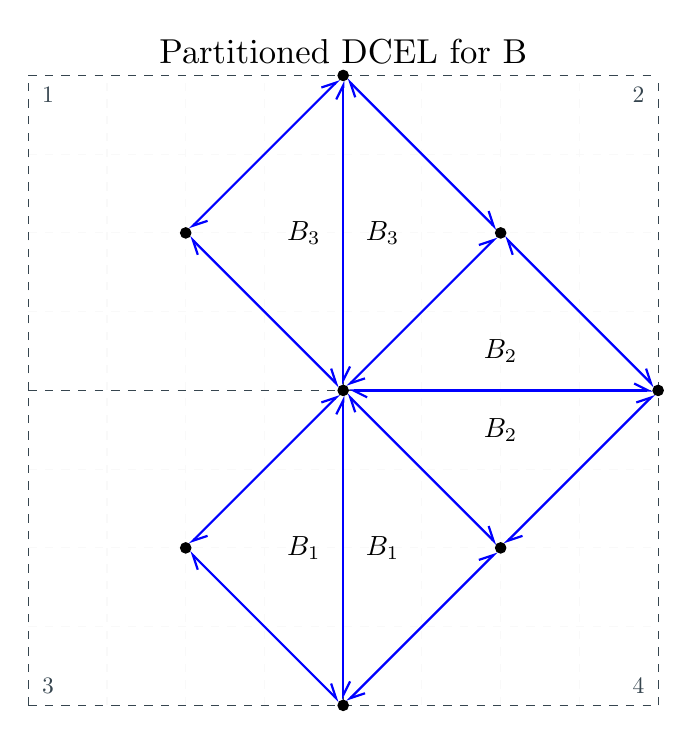
\begin{tikzpicture}
    \tikzstyle{node1}=[draw,scale=0.4,shape=circle,color=black,fill=black]
    \tikzstyle{node2}=[draw,scale=0.4,shape=circle,color=red,fill=red]    
    \draw[color=light-gray, style=dashed] (0,0) grid (8,8);
    \draw[color=pcolor, style=dashed, step=4] (0,0) grid (8,8);
    \node[scale=0.85, color = pcolor] at (0.25, 7.75) {$1$};
    \node[scale=0.85, color = pcolor] at (7.75, 7.75) {$2$};
    \node[scale=0.85, color = pcolor] at (0.25, 0.25) {$3$};
    \node[scale=0.85, color = pcolor] at (7.75, 0.25) {$4$};
    
    \node[above, scale=1.25] at (4,8) {Partitioned DCEL for B};
    \node[node1] (D) at (2,2) {};
    \node[node1] (F) at (2,6) {};
    \node[node1] (J) at (4,0) {};
    \node[node1] (L) at (4,4) {};
    \node[node1] (N) at (4,8) {};
    \node[node1] (Q) at (6,2) {};
    \node[node1] (S) at (6,6) {};
    \node[node1] (T) at (8,4) {};
    \node at (3.5,2) {$B_1$};
    \node at (6,4.5) {$B_2$};
    \node at (3.5,6) {$B_3$};
    \node at (4.5,2) {$B_1$};
    \node at (6,3.5) {$B_2$};
    \node at (4.5,6) {$B_3$};
    
    \draw[barbarrow](D) -- (J); \draw[barbarrow](D) -- (L); 
    \draw[barbarrow](F) -- (N); \draw[barbarrow](F) -- (L);
    \draw[barbarrow](J) -- (Q); \draw[barbarrow](L) -- (Q); 
    \draw[barbarrow](L) -- (S); \draw[barbarrow](N) -- (S); 
    \draw[barbarrow](Q) -- (T); \draw[barbarrow](S) -- (T);
    \draw[barbarrow] (L) -- (T);
    \draw[barbarrow] (L) -- (N);
    \draw[barbarrow] (L) -- (J);
\end{tikzpicture}
\\
\end{tabular}
\end{document}
